\documentclass[11pt,a4paper]{article}
\usepackage[a4paper, margin=1.3in]{geometry}
\usepackage{mathtools}
\usepackage{fancyhdr}
\usepackage{mathrsfs}

\newcommand{\sheetNr}{10}

\pagestyle{fancy}
\fancyhf{}
\lhead{AI Planning}
\rhead{Exercise Sheet \sheetNr}
\lfoot{Axel Perschmann, Tarek Saier, \today}
\rfoot{Page \thepage\ of \pageref{lastpage}}
\renewcommand{\headrulewidth}{0.3pt}
\renewcommand{\footrulewidth}{0.3pt}
\setlength\parindent{0pt}
\newcommand{\h}[0]{\text{--}}

\begin{document}
\begin{center}
\Huge{\textbf{AI Planning}}\\
\LARGE{\textbf{Exercise Sheet \sheetNr}}
\end{center}
\vspace{2cm}
\begin{tabular}{ll}
Date: & \today\\
Students: & Axel Perschmann, Tarek Saier
\end{tabular}

\section*{Exercise 10.1}
\textbf{Iteration i=1}\\
\\
\begin{tabular}{r|cccccc}
prop $p$ & s & b & c & d & e & t\\
\hline
$h^{c_i}_{max}(p)$ & 0 & 1 & 1 & 2 & 2 & 3
\end{tabular}\\
\\
\begin{tabular}{r|cccccc}
action $o$ & $o_1$ & $o_2$ & $o_3$ & $o_4$ & $o_5$ & $o_6$\\
\hline
pcf $D_i(o)$ & s & b & c & e & e & e
\end{tabular}\\
\\
$G_i:$\\
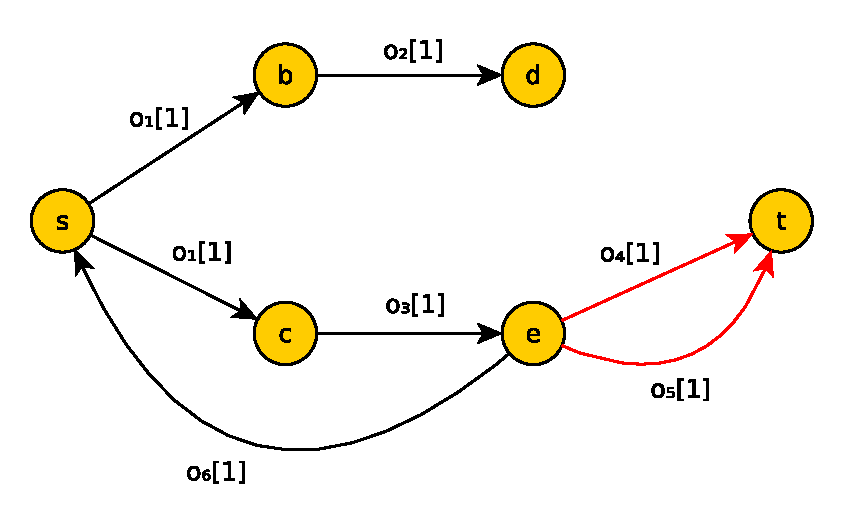
\includegraphics[scale=0.5]{jugraph1}\\
$V^*_i=\{t\}$\\
$V^0_i=\{s,b,c,d,e\}$\\
$V^b_i=\{\}$\\
$L_i=\{o_4,o_5\}$\\
$h_{\text{LM-cut}}(I)$ so far = 1\\
\\
\textbf{Iteration i=2}\\
\\
\begin{tabular}{r|cccccc}
prop $p$ & s & b & c & d & e & t\\
\hline
$h^{c_i}_{max}(p)$ & 0 & 1 & 1 & 2 & 2 & 2
\end{tabular}\\
\\
\begin{tabular}{r|cccccc}
action $o$ & $o_1$ & $o_2$ & $o_3$ & $o_4$ & $o_5$ & $o_6$\\
\hline
pcf $D_i(o)$ & s & b & c & e & e & e
\end{tabular}\\
\newpage
$G_i:$\\
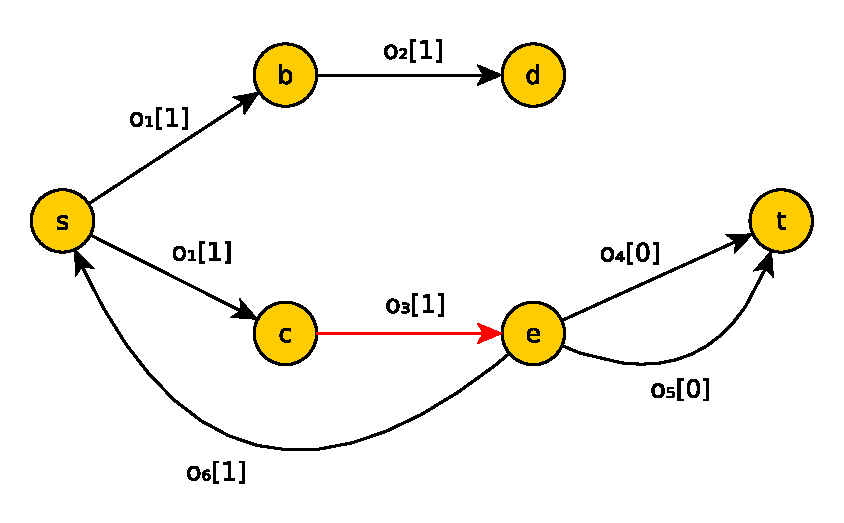
\includegraphics[scale=0.5]{jugraph2}\\
$V^*_i=\{t,e\}$\\
$V^0_i=\{s,b,c,d\}$\\
$V^b_i=\{\}$\\
$L_i=\{o_3\}$\\
$h_{\text{LM-cut}}(I)$ so far = 2\\
\\
\textbf{Iteration i=3}\\
\\
\begin{tabular}{r|cccccc}
prop $p$ & s & b & c & d & e & t\\
\hline
$h^{c_i}_{max}(p)$ & 0 & 1 & 1 & 2 & 1 & 1
\end{tabular}\\
\\
\begin{tabular}{r|cccccc}
action $o$ & $o_1$ & $o_2$ & $o_3$ & $o_4$ & $o_5$ & $o_6$\\
\hline
pcf $D_i(o)$ & s & b & c & e & e & e
\end{tabular}\\
\\
$G_i:$\\
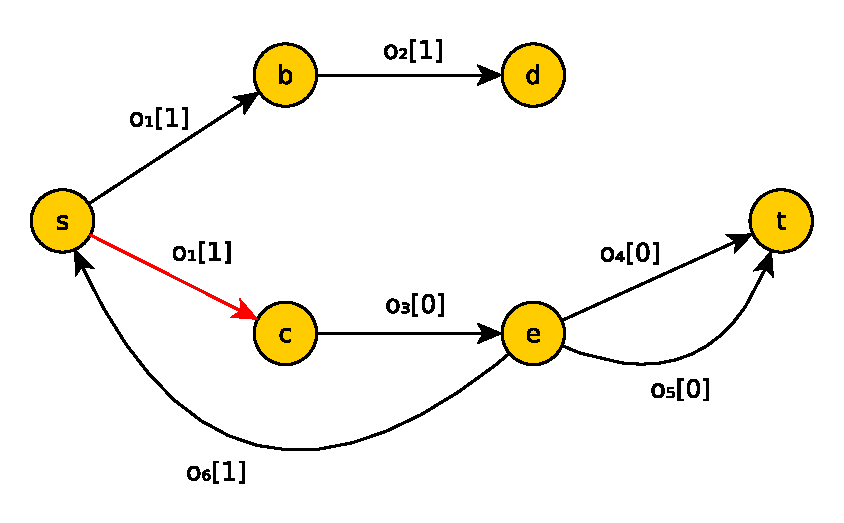
\includegraphics[scale=0.5]{jugraph3}\\
$V^*_i=\{t,e,c\}$\\
$V^0_i=\{s,b,d\}$\\
$V^b_i=\{\}$\\
$L_i=\{o_1\}$\\
$h_{\text{LM-cut}}(I)$ so far = 3\\
\\
\\
\textbf{Iteration i=4}\\
\\
This is when $h^{c_i}_{max}(t)=0$. The task states not to give the pcf, $G_i$, etc. for this iteration.\\
\\
$h_{\text{LM-cut}}(I)=4$

\section*{Exercise 10.2}
\textbf{(a)} \\
\\
\textbf{(b)} \\

\label{lastpage}
\end{document}
